%!TEX root = ../thesis.tex
\chapter{Preliminaries}
\label{preliminaries}

\section{Overview}
\label{preliminaries:overview}

Cryptography is the art and science of secure communication in the presence of third parties. Cryptography is directly related to data privacy and anonymity requirements. The blockchain is a good example of cryptography embracement to enable the sought trust needed for the exchange of digital assets. In this section we review the basic building blocks that cryptography provides to a data sharing system when the blockchain is used. In this Section, cryptographic schemes are introduced in order to lay the ground for the following research. As a result, the exposition style will not be formal in well known cases.

\section{Cryptographic Hash Functions}
\label{preliminaries:hash}

A hash function is a function which takes an input of arbitrary length and returns a fixed-length value~\cite{crypto_101,boneh_crypto,kiagias:crypto,Katz:2014:IMC:2700550}. The hash output value is called digest.

Hash functions have many applications. They are used in data structures -- such as hash tables -- in authentication schemes, password verification and data identifiers to name just a few.

A hash function guarantees at a minimum that for the same input yields the same output. The size of the output is fixed, thus the output range is finite. For this reason it is possible two different inputs produce the same output. This phenomenon is called collision.

Cryptographic hash functions have much stronger properties than regular hash functions. Ideal cryptographic hash functions should be easily computable, noninvertible and collision-resistant~\cite{Katz:2014:IMC:2700550, kiagias:crypto, crypto_101}. A cryptographic hash function $H$ is a deterministic polynomial algorithm that takes as input any given string $x \in \{0, 1\}^{*}$ and outputs a string $H(x) \in \{0, 1\}^{k}$ where $k$ is of fixed size. In the case of a hash function $H$, a collision is a pair of distinct messages $m_0, m_1$ where $m_0 \neq m_1$ and $H(m_0) = H(m_1)$. A hash function $H$ is collision-resistant if it is infeasible for any polynomial-time algorithm to find collisions.

Three levels of security~\cite{Katz:2014:IMC:2700550} can be identified:

\begin{itemize}
  \item Preimage resistance: Given a digest $h$ it is hard to find any message $m$ with $H(m) = h$
  \item Second preimage resistance: For any given message $m_0$ it is hard to find a second message $m_1 \neq m_0$ such as $H(m_0) = H(m_1)$
  \item Collision resistance: It is hard to find a pair of messages $m_0, m_1$ where $m_0 \neq m_1$ and $H(m_0) = H(m_1)$
\end{itemize}

Collision resistance is the strongest security property and a requirement for cryptographic hash functions.

In a data sharing system, cryptographic hash functions can be used to provide file integrity verification and provenance tracking~\cite{10.1109/SPW.2015.27, Azaria2016}. File modifications in transit can be easily detected, as all changes output a different digest. A digest of a dataset serves as a means of unique file identification; unique persistent identifiers (PID) can be used as pointers to a data location. Any change to the PID is visible and trackable~\cite{dist_pid}.

Cryptographic hash functions are heavily used in the blockchain. They are used to create unique transactions and block IDs, to provide proofs of inclusion -- meaning to prove if a transaction is contained in a block -- and, most importantly, to achieve decentralized consensus among the participants. In particular, Bitcoin makes use of the SHA256 and RIPEMD160 hash functions. That said, cryptographic hash functions play an important role in the blockchain ecosystem.

\section{Symmetric-key cryptography}
\label{preliminaries:sym}

In a symmetric cryptosystem two parties share a common secret key agreed prior to communication. The key is used for both encryption and decryption. When a party wants to securely send a message she has to use the secret key to encrypt it and then sent it. The receiver uses the same secret key to decrypt and recover the message. More formally, a symmetric cryptosystem is composed of the following algorithms~\cite{Katz:2014:IMC:2700550, kiagias:crypto}:

\begin{itemize}
  \item A key generation algorithm $\calg$ that takes as input a security parameter $1^{n}$ and outputs a key $k$.
  \item An encryption algorithm $\cale$ that takes as input a key $k$ and a plaintext $m$ and outputs a ciphertext $c$.
  \item A decryption algorithm $\cald$ that takes as input a key $k$ and a ciphertext $c$ and outputs a plaintext $m$.
\end{itemize}

The set of all possible keys which can derive from the key generation algorithm $\calg$ is called the key space $\calk$. Respectively, the set of all possible plaintext is called the plaintext message space denoted $\calm$, and the set of all possible ciphertexts is called ciphertext message space denoted $\calc$. In practice, keys are usually of some fixed length; 256-bit keys are very common. On the other hand, messages and ciphertexts can be of arbitrary length. For example, a message may be a video or a music file or even a single bit.

A symmetric cryptosystem must satisfy the correctness property: for all $m \in \calm$ and $k \in \calk$, it holds that:

\begin{equation*}
  \cald_{k}(\cale_{k}(m)) = m
\end{equation*}

Any deterministic cryptosystem can not be secure~\cite{Katz:2014:IMC:2700550, kiagias:crypto}. For this reason, randomness is essential to any encryption scheme.

In the following chapters the notions of cipher and symmetric encryption scheme or symmetric scheme are identical and will be used interchangeably.

\subsection{Block Ciphers}
\label{preliminaries:sym:block}

A block cipher is a deterministic algorithm that encrypts blocks -- a sequence of bits -- of fixed length. The plaintext and the ciphertext is always of the same size. The size is fixed by the block cipher and is called the \textbf{block size}. The message space $\calm$ and ciphertext space $\calc$ are the same finite set $\{ 0, 1\}^{n}$ and the key space is  $\calk = \{ 0, 1\}^{l}$.

Formally, a block cipher is a keyed permutation function $F: \{ 0, 1\}^{n} \times \{ 0, 1\}^{l} \rightarrow \{ 0, 1\}^{n}$ where $n$ is the block size and $l$ the key size. Usually, the block size and the key size are the same; common key and block sizes range from $128$ to $512$ bits. The function $F$ must be \textbf{one-to-one} for every key $k \in \calk$ and both $F$ and its inverse $F^{-1}$ should be easily computed; there is polynomial-time algorithm that given $k$ computes $F$ and $F^{-1}$. The number of total permutation a block cipher can produce is $2^{n}!$.

The security of a block cipher is much stronger than semantic security~\cite{boneh_crypto}: A permutation produced by $F$ is indistinguishable from a random permutation. Cryptographic schemes based on block ciphers with rigorous proofs of security can, therefore, be constructed.

\begin{figure}[!ht]
    \centering
    \begin{tikzpicture}[node distance=2.5cm,auto,>=latex']
      \node [cipher, minimum size=7em] (a) {AES};
      \draw[<-] (a.west)  -- node[above]{$128$ bits} node[left, xshift=-2em]{$m$} ++(-4em,0em);
      \draw[->] (a.east)  -- node[above]{$128$ bits} node[right, xshift=2em]{$c$} ++(4em,0em);
      \draw[<-] (a.north)  -- node[right]{$128$ bits} node[above, yshift=2em]{$k$} ++(0em,4em);
    \end{tikzpicture}
  \caption{Block cipher AES}
  \label{fig:sym:block:aes}
\end{figure}

\subsubsection[Modes of Operation]{Modes of Operation~\cite{Katz:2014:IMC:2700550}}
\label{preliminaries:sym:modes}

A mode of operation is a way to encrypt arbitrary-length messages using block ciphers of fixed message length. A message is broken into $l$ blocks of size $n$, the block cipher operating on each block. If the size of the last block is less than the block size, the block is padded to a full size block. In most modes of operation, a random initial vector (IV) of length $n$ is required. The IV ensures distinct ciphertexts for each encryption even for the same plaintext and key. The IV is not secret as it is crucial for completing decryption. For a mode to be secure, the IV must be distinct and random in each encryption~\cite{Katz:2014:IMC:2700550}

Several modes of operation are presented below. These modes are vulnerable either to padding oracle attacks~\cite{padding_attacks} -- attacks that exploit the padding validation to decrypt the ciphertext -- or malleable~\cite{malleability} -- the property of transforming one ciphertext into another which decrypts to a different plaintext. To countermeasure padding oracle attacks, or changes to the ciphertext, message authentication~\cite{Katz:2014:IMC:2700550} should be used along with encryption to detect tampering with the ciphertext. Notable modes that combine encryption with authentication are CCM, OCB and GCM.

\epar{Electronic Codebook (ECB)}
\label{preliminaries:sym:modes:ecb}

The Electronic Codebook (ECB) is the simplest mode of operation. Given a plaintext $m = m_1, m_2, \dots, m_l$ each block is encrypted separately. The ciphertext is $c = F_k(m_1), F_k(m_2), \dots, F_k(m_l)$. ECB mode is not secure and should never be used.

\epar{Cipher Block Chaining (CBC)}
\label{preliminaries:sym:modes:cbc}

The Cipher Block Chaining (CBC) mode outputs a sequence of cipher blocks where each plaintext block is XORed with the previous ciphertext block. Each ciphertext is dependent on all preceding blocks. First, a random IV of length $n$ is selected. The first plaintext block is XORed with the IV. The second block is XORed with the first cipher block $c_1$. In general, let $c_0 = IV$ then $c_i = F_k(c_{i-1} \xor m_i) \mbox{, } \forall i \in [1, l]$.

The main drawback of CBC mode is that encryption and decryption are sequential -- meaning that they cannot be parallelized.

\epar{Output Feedback (OFB)}
\label{preliminaries:sym:modes:ofb}

The Output Feedback (OFB) mode uses the block cipher to generate a pseudorandom stream which is then XORed with the plaintext. The stream is generated only by repeatedly encrypting the IV independently of the plaintext. The stream is generated as follows. Set the $i$-th block of the stream to $r_i = F_k(r_{i-1})$ where $r_0 = IV \rselect{\{ 0, 1 \}^{n}}$. The ciphertext is produced by XORing the plaintext with the appropriate stream block; that is, $c_i = m_i \xor r_i$.

As in CBC, the encryption and decryption cannot be parallelized. On the other hand, the pseudorandom stream can be computed independently of the actual message encryption and can be prepared ahead of time.

\epar{Counter (CTR)}
\label{preliminaries:sym:modes:ctr}

The Counter (CTR) mode, like OFB, also generates a pseudorandom stream. First, a random $CTR \rselect{\{ 0, 1 \}^{n}}$ is chosen -- much like the IV in previous modes. The stream is generated as $r_i = F_k(CTR + i)$ where $r_0 = CTR$. Same as before, the ciphertext is computed as $c_i = m_i \xor r_i$.

CTR mode has many advantages. One of the main advantages of CTR mode is that both encryption and decryption can be fully parallelized. Secondly, as with OFB, the stream can be computed in advance. Finally, it is possible to decrypt the $i$-th block of the ciphertext without having to decrypt any other cipher block. This property is called random access.

\begin{figure}[!ht]
    \centering
    \begin{tikzpicture}[node distance=2.5cm,auto,>=latex']
      \node [cipher] (a) {$F_k$};
      \node [cipher, right of=a] (b) {$F_k$};
      \node [cipher, right of=b] (c) {$F_k$};
      \draw[<-] (a.north)  -- node[above, yshift=2em]{$m_1$} ++(0em,4em);
      \draw[<-] (b.north)  -- node[above, yshift=2em]{$m_2$} ++(0em,4em);
      \draw[<-] (c.north)  -- node[above, yshift=2em]{$m_3$} ++(0em,4em);
      \draw[->] (a.south)  -- node[below, yshift=-2em]{$c_1$} ++(0em,-4em);
      \draw[->] (b.south)  -- node[below, yshift=-2em]{$c_2$} ++(0em,-4em);
      \draw[->] (c.south)  -- node[below, yshift=-2em]{$c_3$} ++(0em,-4em);
    \end{tikzpicture}
  \caption{ECB mode}
  \label{fig:sym:block:ecb}
\end{figure}

\begin{figure}[!ht]
    \centering
    \begin{tikzpicture}[node distance=3cm,auto,>=latex']
      \node [cipher] (a) {$F_k$};
      \node [cipher, right of=a] (b) {$F_k$};
      \node [cipher, right of=b] (c) {$F_k$};
      \node [above of=a, node distance=2cm] (xor1) {$\xor$};
      \node [above of=b, node distance=2cm] (xor2) {$\xor$};
      \node [above of=c, node distance=2cm] (xor3) {$\xor$};

      \node[left of=a] (iv) {$IV$};

      \draw[<-] (xor1.north)  -- node[above, yshift=1em]{$m_1$} ++(0em,2em);
      \draw[<-] (a.north)  -- (xor1.south) node[above, yshift=1em]{};

      \draw[<-] (xor2.north)  -- node[above, yshift=1em]{$m_2$} ++(0em,2em);
      \draw[<-] (b.north)  -- (xor2.south) node[above, yshift=1em]{};

      \draw[<-] (xor3.north)  -- node[above, yshift=1em]{$m_3$} ++(0em,2em);
      \draw[<-] (c.north)  -- (xor3.south) node[above, yshift=1em]{};

      \draw[->] (a.south)  -- node[below, yshift=-2em]{$c_1$} ++(0em,-4em);
      \draw[->] (b.south)  -- node[below, yshift=-2em]{$c_2$} ++(0em,-4em);
      \draw[->] (c.south)  -- node[below, yshift=-2em]{$c_3$} ++(0em,-4em);

      \draw[->] (iv.south)  -- node[below, yshift=-2.5em]{$IV$} ++(0em,-5em);

      \draw[->] ([yshift=-4em]a.center) -- ++(3.5em,0em) -- ++(0em,8.7em) -- (xor2.west);
      \draw[->] ([yshift=-4em]b.center) -- ++(3.5em,0em) -- ++(0em,8.7em) -- (xor3.west);

      \draw[->] (iv.north) -- ++(0em, 3.95em) -- (xor1.west);

    \end{tikzpicture}
  \caption{CBC mode}
  \label{fig:sym:block:cbc}
\end{figure}

\begin{figure}[!ht]
    \centering
    \begin{tikzpicture}[node distance=3cm,auto,>=latex']
      \node [cipher] (a) {$F_k$};
      \node [cipher, right of=a] (b) {$F_k$};
      \node [cipher, right of=b] (c) {$F_k$};
      \node [below of=a, node distance=2cm] (xor1) {$\xor$};
      \node [below of=b, node distance=2cm] (xor2) {$\xor$};
      \node [below of=c, node distance=2cm] (xor3) {$\xor$};

      \node[left of=a] (iv) {$IV$};

      \draw[->] (a.south)  -- (xor1.north);
      \draw[->] (xor1.south)  -- node[below, yshift=-1em]{$c_1$} ++(0em,-2em);
      \draw[<-] (xor1.west)  -- node[left, xshift=-1em]{$m_1$} ++(-2em,0em);

      \draw[->] (b.south)  -- (xor2.north);
      \draw[->] (xor2.south)  -- node[below, yshift=-1em]{$c_2$} ++(0em,-2em);
      \draw[<-] (xor2.west)  -- node[left, xshift=-1em]{$m_2$} ++(-2em,0em);
      \draw[->] ([yshift=-3em]a.center) -- ++(3.5em,0em) -- ++(0em,7.7em) --  ++(3.6em,0em) -- (b.north);

      \draw[->] (c.south)  -- (xor3.north);
      \draw[->] (xor3.south)  -- node[below, yshift=-1em]{$c_3$} ++(0em,-2em);
      \draw[<-] (xor3.west)  -- node[left, xshift=-1em]{$m_3$} ++(-2em,0em);
      \draw[->] ([yshift=-3em]b.center) -- ++(3.5em,0em) -- ++(0em,7.7em) --  ++(3.6em,0em) -- (c.north);

      \draw[->] (iv.north) -- ++(0em, 4em) -- ++(7.1em, 0em) -- (a.north);
      \draw[->] (iv.south)  -- node[below, yshift=-3.5em]{$IV$} ++(0em,-6em);

    \end{tikzpicture}
  \caption{OFB mode}
  \label{fig:sym:block:ofb}
\end{figure}

\begin{figure}[!ht]
    \centering
    \begin{tikzpicture}[node distance=3cm,auto,>=latex']
      \node [cipher] (a) {$F_k$};
      \node [cipher, right of=a] (b) {$F_k$};
      \node [cipher, right of=b] (c) {$F_k$};
      \node [below of=a, node distance=2cm] (xor1) {$\xor$};
      \node [below of=b, node distance=2cm] (xor2) {$\xor$};
      \node [below of=c, node distance=2cm] (xor3) {$\xor$};

      \draw[<-] (a.north)  -- node[above, yshift=1em]{$CTR + 1$} ++(0em,2em);
      \draw[<-] (b.north)  -- node[above, yshift=1em]{$CTR + 2$} ++(0em,2em);
      \draw[<-] (c.north)  -- node[above, yshift=1em]{$CTR + 3$} ++(0em,2em);

      \node[left of=a] (iv) {$CTR$};

      \draw[->] (a.south)  -- (xor1.north);
      \draw[->] (xor1.south)  -- node[below, yshift=-1em]{$c_1$} ++(0em,-2em);
      \draw[<-] (xor1.west)  -- node[left, xshift=-1em]{$m_1$} ++(-2em,0em);

      \draw[->] (b.south)  -- (xor2.north);
      \draw[->] (xor2.south)  -- node[below, yshift=-1em]{$c_2$} ++(0em,-2em);
      \draw[<-] (xor2.west)  -- node[left, xshift=-1em]{$m_2$} ++(-2em,0em);

      \draw[->] (c.south)  -- (xor3.north);
      \draw[->] (xor3.south)  -- node[below, yshift=-1em]{$c_3$} ++(0em,-2em);
      \draw[<-] (xor3.west)  -- node[left, xshift=-1em]{$m_3$} ++(-2em,0em);

      \draw[->] (iv.south)  -- node[below, yshift=-3.5em]{$CTR$} ++(0em,-6em);

    \end{tikzpicture}
  \caption{CTR mode}
  \label{fig:sym:block:ctr}
\end{figure}

\section{Public Key Cryptography}
\label{preliminaries:pub}

As we see in~\ref{preliminaries:sym} a secret key has to been agreed prior to communication. In 1976, Whitfield Diffie and Martin Hellman published a paper called New Directions in Cryptography~\cite{Diffie:2006:NDC:2263321.2269104} that changed the way of communication. They proposed a protocol that enables two parties, having no prior communication, to establish a secret key over an insecure channel in the presence of eavesdropping adversaries. The protocol uses two keys, one for encryption and one for decryption. The encryption key is called the public key and the decryption key is called the secret key (or private). Every party has a key pair consisting of a public and a secret key. The public key is made available for anyone---the receiver may post the public key online beforehand---that want to sent an encrypted message to the holder of the corresponding secret key. The receiver of the message decrypts the ciphertext with the use of her private key. Only the owner of the private key can decrypt a message that was encrypted with the corresponding public key. In an essence, a key pair is an identity and the blockchain smartly utilizes it to provide anonymous identities to the users of the system.

More formally, a public-key encryption scheme is composed of the following probabilistic, polynomial-time algorithms~\cite{Katz:2014:IMC:2700550, kiagias:crypto}:

\begin{itemize}
  \item The key generation algorithm $\calg$: Take as input a security parameter $1^{n}$ it and outputs a key pair ($p_k$, $s_k$).
  \item The encryption algorithm $\cale$: Take as input a public key $p_k$ and a plaintext $m$ and outputs a ciphertext $c$.
  \item The decryption algorithm $\cald$: Take as input a private key $s_k$ and a ciphertext $c$ and outputs a plaintext $m$.
\end{itemize}

Likewise, a public-key cryptosystem must satisfy the correctness property: for all $m \in \calm$ and $(p_k, s_k) \in \calk$, it holds that

\begin{equation*}
  \cald_{s_k}(\cale_{p_k}(m)) = m
\end{equation*}

Many important and wide-used public-key schemes base their security on mathematical problems that, under certain conditions, are assumed to be hard; they cannot be solved in polynomial time. Such problems are the discrete logarithm and the factoring problem.

\subsection[Discrete Logarithm and Diffie-Hellman Assumptions]{Discrete Logarithm and Diffie-Hellman Assumptions~\cite{Katz:2014:IMC:2700550, kiagias:crypto}}
\label{preliminaries:pub:dlog}

In cryptography, any system to be considered secure has to be provable secure. There are cryptosystems which are perfectly secure~\cite{shannon_otp}, such as the one-time pad~\cite{shannon_otp}, and others that perfect security cannot be achieved. In such case, the security is proven by computational security assumptions; reductions to a particular problem which is assumed, under certain conditions, to be hard to solve in polynomial-time. The discrete log problem is one of those problems and significant cryptographic schemes, such as the Diffie-Hellman key exchange and El Gamal encryption and signature protocol, was built under the discrete log computational hardness assumption.

\begin{dfn}
  Let $\G$ be a cyclic group of order $q$ and let $g$ be a generator of $\G$. The \textbf{discrete log problem} (DLOG) is as follows: given a random element $h \in \G$, find an integer $x \in \Z_q$ such that $g^{x} = h$.
\end{dfn}

\begin{dfn}
 The \textbf{computational Diffie-Hellman problem} (CDH) is as follows: given a cyclic group $\G$ of order $q$, a generator $g \in \G$, $g^{a}$ and $g^{b}$ where $a, b \rselect{\Z_q}$, compute $g^{ab}$.
\end{dfn}

\begin{dfn}
 The \textbf{decisional Diffie-Hellman problem} (DDH) is as follows: given a cyclic group $\G$ of order $q$, a generator $g \in \G$, and $g^{a}, g^{b}, g^{c}$ where $a, b, c \rselect{\Z_q}$, decide if $c = ab$ or $c \rselect{\Z_q}$.
\end{dfn}

The DLOG problem is believed to be hard for specific group families of $\G$. For example, solving the DLOG for the subgroup of order $q$ of $\Z^{*}_{p}$, where $p$ and $q$ are primes of size at least $2048$-bits and $256$-bits respectively, is considered infeasible. This assumption is called the \textbf{discrete log assumption}.

The DDH problem is weaker than the CDH problem and it holds that $DDH \leq CDH$; If an adversary could solve CDH, she can compute $g^{ab}$ and comparing it to $g^{c}$ and easily solves the DDH.

\section{Digital signatures}
\label{preliminaries:sign}

A digital signature is a fundamental cryptographic primitive. It can be considered as the equivalent to a handwritten signature. It is a scheme from presenting the authenticity of digital messages or documents.

In a digital signature scheme, each party holds a unique key pair $(p_k, s_k)$. The signing key $s_k$ is used to uniquely sign a message $m$ and the verification key $p_k$ to verify the signature. Only someone with knowledge of $s_k$ can sign a message, but all parties having access to $p_k$ can verify a signature.

Digital signatures have the following important properties:

\begin{itemize}
  \item Authentication: The message was signed by a known sender
  \item Non-repudiation: The sender cannot deny having sent the message
  \item Integrity: The message was not altered in transit
\end{itemize}

Digital signatures are commonly used for software distribution and financial transactions and in cases where forgery detection is important. Blockchain is empowered with digital signatures to provide asset ownership; the rightful owner sign the transaction to prove possession of the asset.

More formally, a digital signature scheme is composed of the following probabilistic polynomial-time algorithms~\cite{Katz:2014:IMC:2700550,kiagias:crypto}:

\begin{itemize}
  \item The key generation algorithm $Gen$: Take as input a security parameter $1^{n}$ and outputs a key pair ($p_k$, $s_k$).
  \item A signing algorithm $Sign$: Take a signing key $s_k$ and a message $m$ and produce a digital signature $\sigma$ of $m$
  \item A deterministic verification algorithm $Verify$: Take a verification key $p_k$ and a signature $\sigma$. It outputs $b=1$ or $b=0$ ($true$ or $false$) to indicate if the signature is valid.
\end{itemize}

The primary goal of digital signatures is unforgeability; an adversary cannot create a new valid message-signature pair without the corresponding signing key.

\subsection{El Gamal Signature Scheme}
\label{preliminaries:sign:el_gamal}

The El Gamal Signature Scheme~\cite{el_gamal} is a digital signature scheme based on the difficulty of the discrete logarithm problem (§~\ref{preliminaries:pub:dlog}).

The scheme works as follows:

\begin{itemize}
  \item Key Generation:
    \begin{enumerate}
      \item Choose a cryptographic hash function $H$ where $H: \{0, 1\}^{*} \rightarrow \{0, 1\}^{n}$
      \item Choose a prime $p$ such as the DLOG problem is difficult
      \item Find a generator $g$ of the group $\Z^{*}_{p}$
      \item Choose randomly $x \rselect{\Z_q}$
      \item Compute $h = g^{x} modp$
      \item Return $(h, x)$ where $h$ is the public key and $x$ the private key
    \end{enumerate}
  \item Sign: Sign a message $m \in \{0, 1\}^{*}$ with a private key $x$
    \begin{enumerate}
      \item Choose randomly $k \rselect{\Z_q}$ such that $gcd(k, p - 1) = 1$
      \item Compute $r = g^{k}modp$
      \item Compute $s = k^{-1}(H(m) + xr) mod(p - 1)$
      \item Return the signature $(r, s)$
    \end{enumerate}
  \item Verify: Verify a signature $(r, s)$ of the message $m$ with a public key $h$
    \begin{enumerate}
      \item Verify that $r \in \Z_q$ and $s \in \Z_q$. Else ouput $0$.
      \item Compute $v = H(m)$
      \item If $v \stackrel{?}{=} (h^{r}r^{s}) modp$ then output $1$ else $0$.
    \end{enumerate}
\end{itemize}

\subsection{Digital Signature Algorithm (DSA)}
\label{preliminaries:sign:dsa}

The Digital Signature Algorithm (DSA)~\cite{dsa_nist} has been standardised by the National Institute of Standards and Technology (NIST). DSA is a variant of the El Gamal signature scheme. The main advantage of DSA over El Gamal Signature is the size of the signature. DSA produce signatures of size $320$-bit in comparison to El Gamal that needs at least signatures of size $2048$-bit to be secure given todays security standards~\cite{dsa}.

The algorithm work as follows~\cite{dsa}:

\begin{itemize}
  \item Key Generation:
    \begin{enumerate}
      \item Choose a cryptographic hash function $H$ where $H: \{0, 1\}^{*} \rightarrow \{0, 1\}^{n}$
      \item Choose a prime $q$ of size $n$
      \item Choose a prime $p$ such that $p - 1$ is a multiple of $q$ of size $l$. The size of $l$ must be a multiple of $64$ between $512$ and $1,024$
      \item Choose randomly $a \rselect{\Z_p}$
      \item Compute $g = a^{(p - 1)/q} mod p$
      \item Choose randomly $x \rselect{\Z_q}$
      \item Compute $h = g^{x} modp$
      \item Return $((p, q, g), h, x)$ where $(p, q, g)$ is the public parameters of the algorithm, $h$ is the public key and $x$ the private key.
    \end{enumerate}
  \item Sign: Sign a message $m \in \{0, 1\}^{*}$ with a private key $x$
    \begin{enumerate}
      \item Choose randomly $k \rselect{\Z_q}$
      \item Compute $r = (g^{k}modp)modq$
      \item Compute $s = k^{-1}(H(m) + xr) modq$
      \item Return the signature $(r, s)$
    \end{enumerate}
  \item Verify: Verify a signature $(r, s)$ of the message $m$ with a public key $h$
    \begin{enumerate}
      \item Verify that $r \in \Z_q$ and $s \in \Z_q$. Else ouput $0$.
      \item Calculate $w = s^{-1}modq$
      \item Calculate $u_1 = (H(m)w)modq$
      \item Calculate $u_2 = (rw)modq$
      \item Calculate $v = ((g^{u_1}h^{u_2})modp)modq$
      \item If $v \stackrel{?}{=} r$ then output $1$ else $0$.
    \end{enumerate}
\end{itemize}

\section{Elliptic-curves}
\label{preliminaries:el_curves}

Elliptic curves (ECC) play an import role in cryptography. All cryptosystems, defined in previous chaptes, are built over multiplicative groups of integers modulo a sufficient large prime $p$~\cite{kiagias:crypto, boneh_crypto}. Elliptic curves are additive abelian groups~\cite{kiagias:crypto}; a group satisfying associativity, commutativity, existence of identity element and inverse under the addition group operation~\cite{elliptic_curves_2}.

There are two apparent benefits for using curves over modular groups~\cite{kiagias:crypto}. The first is cost efficiency. In practice, cryptosystems that their security depends on the discrete log problem or the factorisation problem on a modular group, such as the El Gamal or the RSA, the primes have to be at least 2048 bits for the system to be secure. On the other hand, elliptic curves offer similar security using much smaller key sizes. A 233-bit elliptic curve key gives the same level of security as a 2,240-bit RSA key~\cite{ecc_rsa_bits, ecc_rsa_bits_1} and a 333-bit elliptic curve key as a 4096-bit RSA key~\cite{blake1999elliptic}. The second reason is that, for the moment, there is no know way to generalise the attacks against the discrete logarithm problem on a modular group to elliptic curves~\cite{kiagias:crypto}.

Cryptography is primarily interested in elliptic curves over $\F_p$: the field of integers modulo $p$ where $p$ is a prime number. An elliptic curve $E$ over $\F_p$ is defined by the equation of the form~\cite{elliptic_curves, elliptic_curves_2}:

\begin{equation*}
  y^2 = x^3 + ax + b
\end{equation*}

where $a, b \in \F_p$. A pair $(x, y)$ where $x, y \in \F_p$ is a point on the curve if it satisfies the equation where $E$ is defined. There is a special point, called \textbf{point at infinity} and denoted by $\infty$, where is also on the curve and serve as the identity element~\cite{elliptic_curves_2}.

\begin{figure}
  \centering
  \begin{tikzpicture}
    \begin{axis}[
            xmin=-4,
            xmax=5,
            ymin=-5,
            ymax=5,
            xlabel={$x$},
            ylabel={$y$},
            scale only axis,
            axis lines=middle,
            domain=-1.3247:2,
            y domain=-3:3,
            samples=200,
            smooth,
            clip=false,
            axis equal image=false,
            ticks=none
        ]

    \addplot[red] {sqrt(x^3-x+1)} node[right, black] {$y^2 = x^3 - x + 1$};
    \addplot[red] {-sqrt(x^3-x+1)};

    \end{axis}
    \end{tikzpicture}
  \caption{Elliptic curve}
\end{figure}

\subsection[Points addition]{Points addition~\cite{elliptic_curves}}
\label{preliminaries:el_curves:addition}

Let $P = (x_1, y_1)$ and $Q = (x_2, y_2)$ two points on the elliptic curve $E$ where $P \neq Q$ and $P, Q \neq \infty$. Any two points on a curve add to produce a third point on the curve. A third point $R = (x_3, y_3)$ on the curve $E$ is defined as:

\begin{equation*}
  R = P + Q
\end{equation*}

We can find the third point $R$ as follows:

\begin{enumerate}
  \item Draw the line $L$ through $P$ and $Q$.
  \item Find the third point $-R$ that $L$ intersects with.
  \item Reflect $-R$ across the $x$-axis to obtain $R$
\end{enumerate}

The slope of the line $L$ can be found as

\begin{equation*}
  m = \dfrac{y_2 - y_1}{x_2 - x_1}
\end{equation*}

and assuming $x_1 \neq x_2$ the equation of $L$ is

\begin{equation*}
  y = m(x - x_1) + y_1
\end{equation*}

To find the intersection with $E$, substitute $y$ to get

\begin{equation*}
  (m(x - x_1) + y_1)^{2} = x^3 + ax + b
\end{equation*}

The three roots of cubic polynomial correspond to the three points of intersection of $L$ with $E$. As we already know the two of the tree roots, since $P$ and $Q$ are points on both $L$ and $E$, finding the third root is easy. For a cubic polynomial $x^{3} + ax^{2} + bx + c$ with roots $r, s, t$ it holds that~\cite{elliptic_curves}

\begin{equation*}
  x^{3} + ax^{2} + bx + c = (x - r)(x - s)(x - t) = x^{3} - (r + s + t)x^{2} + \dots
\end{equation*}

Therefore,

\begin{equation*}
  r + s + t = -a
\end{equation*}

Knowing the two roots $r, s$ we can recover the third as $t = -a - r  - s$.

So, to find the third point where $L$ intersects with $E$ we obtain

\begin{equation*}
  x = m^{2} + - x_1 - x_2
\end{equation*}

and

\begin{equation*}
  y = m(x - x_1) + y_1
\end{equation*}

Finally, to reflect $-R$ to the $x$-axis to obtain $R$ we change the sign of $y_1$. The final equations that give the third point are

\begin{align*}
  x_3 = m^{2} + - x_1 - x_2, && y_3 = m(x_1 - x_3) - y_1
\end{align*}

\begin{figure}
  \centering
  \begin{tikzpicture}
    \begin{axis}[
            xmin=-4,
            xmax=5,
            ymin=-5,
            ymax=5,
            xlabel={$x$},
            ylabel={$y$},
            scale only axis,
            axis lines=middle,
            domain=-1.3247:2,
            y domain=-3:3,
            samples=200,
            smooth,
            clip=false,
            axis equal image=false,
            ticks=none,
        ]

    \addplot[red] {sqrt(x^3-x+1)} node[right, black] {};
    \addplot[red] {-sqrt(x^3-x+1)};
    \addplot[blue, domain=-3:3,] {0.27*x + 0.87};

    \draw [fill=black] (axis cs:-1.25, 0.535) circle (2pt);
    \draw [fill=black] (axis cs:0.165, 0.9) circle (2pt);
    \draw [fill=black] (axis cs:1.165, 1.17) circle (2pt);
    \draw [fill=black] (axis cs:1.165, -1.17) circle (2pt);

    \draw [dashed] (axis cs:1.165, 1.17) -- (axis cs:1.165,-1.17);

    \draw[color=black] (axis cs:-1.4, 0.635) node [left]{$P$};
    \draw[color=black] (axis cs:0.0, 1.5) node [left]{$Q$};
    \draw[color=black] (axis cs: 1.4, 1.6) node [left]{$-R$};
    \draw[color=black] (axis cs: 3.7, -1) node [left]{$R = P + Q$};

    \end{axis}
    \end{tikzpicture}
  \caption{Addition of points on elliptic curves}
\end{figure}

\subsection[Points doubling]{Points doubling~\cite{elliptic_curves}}
\label{preliminaries:el_curves:doubling}

Let $P = (x_1, y_1)$ a points on the elliptic curve $E$ where $P \neq -P$ and $P \neq \infty$. Then $2P = (x_3, y_3)$. Unlike ~\ref{preliminaries:el_curves:addition}, where we have two points, in point doubling we have only one point, thus we cannot draw the line $L$. In that case, we use the tangent line $L$ to the curve $E$ at point $P$.

The slope of $L$ can be found as

\begin{equation*}
  m = \dfrac{dy}{dx} = \dfrac{3x_1^{2} + a}{2y_1}
\end{equation*}

Assuming $y_1 \neq 0$ the equation of $L$ is

\begin{equation*}
  y = m(x - x_1) + y_1
\end{equation*}

Therefore, proceeding as in~\ref{preliminaries:el_curves:addition}, we obtain

\begin{align*}
  x_3 = m^{2} + - 2x_1, && y_3 = m(x_1 - x_3) - y_1
\end{align*}

\subsection{Elliptic curve discrete logarithm problem (ECDLP)}

As with multiplicative groups, cyclic subgroups of some such elliptic curve groups can be used to implement secure systems based on the discrete logarithm problem which is as well assumed to be hard.

\begin{dfn}
  The elliptic curve discrete logarithm problem (ECDLP) is as follows: given an elliptic curve $E$ over a finite field $\F_p$ and two points $P, Q \in E$, find an integer $d \in \Z_p$ such that $Q = dP$.
\end{dfn}

The parameters that describe an elliptic curve $E$ defined over a finite field $\F_p$, a base (generator) point $P \in E$, and its order $q$ should be chosen carefully so that the ECDLP is resistant to all known attacks.

\subsection[Key generation]{Key generation~\cite{elliptic_curves_2}}
\label{preliminaries:el_curves:key_gen}

Let $E$ be an elliptic curve over $\F_p$ and $P$ a generator point in $E$ of order $q$. The key pair generation algorithm is defined as follows:

\begin{enumerate}
  \item Select a random integer $d \rselect{\in \Z_q}$
  \item Compute $Q = dP$
  \item Return the tuple $(Q, d)$ where $Q$ is the public key and $d$ the secret key
\end{enumerate}

The prime $p$, the curve $E$ the generator point $P$, its order $q$ and the public key $Q$ are public and finding the secret key $d$ is equivalent to solving the ECDLP.

\subsection{Elliptic Curve Digital Signature Algorithm (ECDSA)}
\label{preliminaries:sign:el_curves:ecdsa}

The Elliptic Curve Digital Signature Algorithm (ECDSA)~\cite{ecdsa} is a variant of the Digital Signature Algorithm (DSA) which use elliptic Curves. It is the most widely standardized elliptic curve-based signature scheme~\cite{elliptic_curves_2}.

Let $E$ be an elliptic curve over $\F_p$, a generator point $P$ of order $q$ and $H$ a cryptographic hash function where $H: \{0, 1\}^{*} \rightarrow  \{0, 1\}^{q}$. The ECDSA is defined as follows~\cite{elliptic_curves_2}:

\begin{itemize}
  \item Key generation: Run elliptic curve key generation algorithm defined in~\ref{preliminaries:el_curves:key_gen} and get a key pair $(Q, d)$.
  \item Sign: Sign a message $m$ with a private key $d$
    \begin{enumerate}
      \item Choose randomly $k \rselect{\Z_q}$
      \item Compute the point $kP = (x_1, y_1)$
      \item Compute $r = x_1modq$. If $r \stackrel{?}{=} 0$ then go to step 1
      \item Compute $e = H(m)$
      \item Compute $s = k^{-1} (e + dr) modq$. If $s \stackrel{?}{=} 0$ then go to step 1
      \item Return the signature $(r, s)$
    \end{enumerate}
  \item Verify: Verifies a signature $(r, s)$ of the message $m$ with a public key $Q$
    \begin{enumerate}
      \item Verify that $r \in \Z_q$ and $s \in \Z_q$. Else ouput $0$.
      \item Compute $e = H(m)$
      \item Compute $w = s^{-1}modq$
      \item Compute $u_1 = (ew)modq$ and $u_2 = (rw)modq$
      \item Compute $X = u_1P + u_2Q$
      \item If $X \stackrel{?}{=} \infty$ output $0$
      \item Take $x_1$ cordinate of $X$ and compute $v = x_1modq$
      \item If $v \stackrel{?}{=} r$ then output $1$ else $0$.
    \end{enumerate}
\end{itemize}

Blockchain uses elliptic curves for key pair generation and transaction signing (ECDSA). Bitcoin and Ethereum use a specific elliptic curve for ECDSA~\cite{ecdsa} which its parameters are defined in the secp256k1 standard~\cite{secp}.

\section{Homomorphic Encryption}
\label{preliminaries:homo}

Homomorphic encryption allows specific types of computation on encrypted data. It allows to perform computations over ciphertexts and return encrypted results that when decrypted matches the result of the operations as if they had been performed on the plaintext. An encryption scheme is called homomorphic when it has the homomorphic property. In particular, if for all $m_1, m_2 \in \calm$ and $k \in \calk$ (secret key or public key):

\begin{equation*}
  Enc_k(m_1) \otimes Enc_k(m_2) = Enc_k(m_1 \oplus m_2)
\end{equation*}

then the encryption scheme is homomorphic.

Homomorphic encryption schemes are by nature malleable and have weaker security properties than non-homomorphic schemes. Various known encryption schemes are homomorphic such as the unpadded RSA and El Gamal.

\section{Zero Knowledge Proofs}
\label{zkp}

A proof of knowledge is a protocol that enables one party to convince another of the validity of a statement.
In a zero-knowledge proof~\cite{zkp}, this is accomplished without revealing any information beyond the legitimacy of the proof~\cite{kiagias:crypto},
meaning that one party can prove to another party that a given statement is true, without conveying any information apart from the fact that the statement is indeed true.

Let $\calp$ be a prover and $\calv$ the verifier. $\calp$ must convince $\calv$ that she has some
knowledge of a statement $x$ without explicitly stating what she knows. We call this knowledge a witness $w$.
Both parties are aware of a predicate $R$ that will attest to $w$ being a valid witness to $x$~\cite{kiagias:crypto}. In general,

\begin{itemize}
  \item The predicate $R$ is assumed to be polynomial-time computable.
  \item The prover $\calp$ has $R,x$, and $w$ such that $R(x,w) = 1$. She wishes to prove possesion of $w$ by producing a proof of knowledge $\pi$.
  \item The verifier $\calv$ has $R,x$, and $\pi$.
  \item Given $R$ it is hard to find a corresponding $w$ such as $R(x,w) = 1$
  \item The prover $\calp$ is unwilling to reveal $w$; otherwise the solution is trivial.
  \item The verifier $\calv$ can efficiently check the validity of $\pi$.
\end{itemize}

\subsection{Examples}

\subsubsection{The strange cave of Ali Baba}
\label{zkp:examples}

Let's bring our old friends Alice and Bob and define the following game: at the bottom of the cave~\cite{Quisquater:1989:EZP:118209.118269} of figure~\ref{fig:zkp:alibaba} there is a magic door that
can only be open using a secret password. The cave is shaped like a rectangle with one entrance at one side and the magic door blocking the opposite side. Bob knows the secret password and wants to prove to Alice that he can open the magic door without revealing the password to Alice.
Bob propose the following game to prove to Alice he can open the magic door: Alice waits outside the cave, Bob enters the cave and
takes either from the left or right path. Alice can not see which path Bob takes. Then Alice enters, stands at the entrance of cave and calls
Bob to come out either the left or the right passage. Bob complies, using the secret password if necessary.

If Bob does not know the secret password he has $1/2$ change of guessing correctly as Alice choose at random which path Bob should take. If they repeat this procedure $k$ times the probability of Bob convincing Alice that he knows the secret password without actually knowing it reduce exponentially; at most $1/2^{k}$.

\subsubsection{The colour-blind friend}

Let's bring again our friends Alice and Bob. Suppose Bob is color-blind~\cite{zkp:colour_blind} and Alice has two balls: one red and one green but otherwise identical when you touch them.
To Alice they seem complete identical and she is not sure if they are actually distinguishable. Bob wants to prove to Alice that indeed the are differently-coloured
without revealing which one is red and which is green. To prove his knowledge, Bob gives to Alice the two balls so that she is holding one in each hand. Bob can see
at this point which ball is in which hand. Next, Alice either switches the ball behind her hands or leaves them be, with probability $1/2$. Finally, she brings
them out from behind her back. Alice then asks Bob if she switch the balls. By looking at their colors, Bob can can say with certainty whether he switched them or not.
On the other hand, if they were the same color and hence indistinguishable, there is no way he could guess correctly with probability higher than 1/2. If they repeat
this procedure $k$ times the probability that Bob succeeded at identifying all the tries when the balls are identical is at most $1/2^{k}$.

\begin{figure}[t!]
  \centering
  \begin{subfigure}[t]{0.30\textwidth}
    \centering
    \resizebox{\linewidth}{!}{
      \begin{tikzpicture}[scale=1]
        % Cave %
        \draw(0,5) -- (2,5) -- (2,8) -- (10,8) -- (10,4);
        \draw(0,4) --(2,4) -- (2,1) -- (10,1) -- (10, 4);
        \draw(9,4.5) -- (10,4.5);
        \draw(3,5) -- (3,7) -- (9,7) -- (9,5);
        \draw(3,5) -- (3,2) -- (9,2) -- (9,5);
        % Actors %
        \draw[fill] (1,5.6) circle [radius=0.1];
        \node [below] (alice) at (1,5.5) {Alice};
        \draw[fill] (2.5,4.6) circle [radius=0.1];
        \node [below] (bob) at (2.5,4.5) {Bob};
        % Arrows %
        \draw [dashed, ->] (2.5,4.6) -- (2.5,6);
        \draw [dashed, ->] (2.5,3.9) -- (2.5,2);

      \end{tikzpicture}
    }
    \caption{Alice stands outside and Bob choose randomly a path, left or right}
    \label{fig:zkp:alibaba:a}
  \end{subfigure}
  \begin{subfigure}[t]{0.30\textwidth}
    \centering
    \resizebox{\linewidth}{!}{
      \begin{tikzpicture}[scale=1]
        % Cave %
        \draw(0,5) -- (2,5) -- (2,8) -- (10,8) -- (10,4);
        \draw(0,4) --(2,4) -- (2,1) -- (10,1) -- (10, 4);
        \draw(9,4.5) -- (10,4.5);
        \draw(3,5) -- (3,7) -- (9,7) -- (9,5);
        \draw(3,5) -- (3,2) -- (9,2) -- (9,5);
        % Actors %
        \draw[fill] (2.5,4.6) circle [radius=0.1];
        \node [below] (alice) at (2.5,4.5) {Alice};
        \draw[fill] (9.5,4.3) circle [radius=0.1];
        \node [below] (bob) at (9.5,4.2) {Bob};
        % Speech Bubble %
        \node[overlay,draw,cloud callout,callout relative pointer={(0.2cm,-0.7cm)},%
        aspect=2.5,fill=white!90] at ($(alice)+(-0.5cm,2.3cm)$) {Left};

      \end{tikzpicture}
    }
    \caption{Alice calls to Bob, asking him to come out either the left or the right passage}
    \label{fig:zkp:alibaba:b}
  \end{subfigure}
  \begin{subfigure}[t]{0.30\textwidth}
    \centering
    \resizebox{\linewidth}{!}{
      \begin{tikzpicture}[scale=1]
        % Cave %
        \draw(0,5) -- (2,5) -- (2,8) -- (10,8) -- (10,4);
        \draw(0,4) --(2,4) -- (2,1) -- (10,1) -- (10, 4);
        \draw(9,4.5) -- (9.5,4.5);
        \draw(3,5) -- (3,7) -- (9,7) -- (9,5);
        \draw(3,5) -- (3,2) -- (9,2) -- (9,5);
        % Actors %
        \draw[fill] (2.5,4.6) circle [radius=0.1];
        \node [below] (alice) at (2.5,4.5) {Alice};
        \draw[fill] (2.5,7.8) circle [radius=0.1];
        \node [below] (bob) at (2.5,7.7) {Bob};
        % Speech Bubble %
        \node[overlay,draw,cloud callout,callout relative pointer={(0.2cm,-0.7cm)},%
        aspect=2.5,fill=white!90] at ($(alice)+(-0.5cm,2.3cm)$) {OK};

      \end{tikzpicture}
    }
    \caption{Bob complies appearing at the exit Alices names}
    \label{fig:zkp:alibaba:c}
  \end{subfigure}
  \caption{Ali Baba Cave}
  \label{fig:zkp:alibaba}
\end{figure}

\subsection[Formal Definition]{Formal Definition~\cite{kiagias:crypto}}
\label{zkp:definition}

Let $<\calp, \calv>$ be a pair of interactive programs. Define $\text{out}^{\calp}_{\calp, \calv}(x,w,z)$
to be the output of $\calp$ when both $\calp$ and $\calv$ are executed with the public input $x$ and private
inputs $w$ and $z$ ($\calp$ determines $w$ and $\calv$ choose $z$); $\text{out}^{\calv}_{\calp, \calv}(x,w,z)$
is similar defined for $\calv$. The PPT interactive protocol $<\calp, \calv>$ is a \textbf{zero-knowledge proof}
for a language $L \in NP$ with knowledge error $k$ and zero-knowledge distance $\e$ if the following
properties hold~\cite{kiagias:crypto}.

\begin{enumerate}
  \item \textbf{Completeness:} If $x \in L$ and $R(x,w) = 1$ for some witness $w$, then $\text{out}^{\calv}_{\calp, \calv}(x,w,z)$ = 1
    for all string $z$ with overwhelming probability in $v$.
  \item \textbf{Soundness:} For any polynomial-time program $\calp^{*}$ define for arbitrary $x,w,z,$
    \begin{equation*}
      \pi_{x,w,z} = \Prob[\text{out}^{\calv}_{\calp^{*}, \calv}(x,w,z) = 1].
    \end{equation*}
    A protocol $<\calp, \calv>$ satisfies soundness if there are non-negligible functions $s(v), q(v)$ such for all $\calp^{*}$ here exists a probabilistic
    Turing machine (PTM) program $K$, called a knowledge extractor with the following property. Suppose that

    \begin{equation*}
      \widetilde{\pi} = \Prob[K(x,w,z) = w^{'} : R(x, x^{'}) = 1].
    \end{equation*}
    Then it holds that $\pi_{x,w,z} \geq s(|x|)$ implies that $\widetilde{\pi}_{x,w,z} \geq q(\abs{x})$.

  \item \textbf{(Statistical) Zero-knowledge:} For each polynomial-time program $\calv^{*}$, there is a PTM program $S$, called the \textbf{simulator}, such that for all
    $x,w$ with $R(x,w) = 1$, the random variables $S(x,z)$ and $\text{out}^{\calv^{*}}_{\calp, \calv^{*}}(x,w,z)$ are statistically indistinguishable for all strings $z$:
    \begin{equation*}
      \forall \cala \abs[\Big]{\Prob[\cala(S(x,z) = 1)] - \Prob[\cala(\text{out}^{\calv^{*}}_{\calp, \calv^{*}}(x,w,z)) = 1]} < \e.
    \end{equation*}
\end{enumerate}

Completeness is very similar to correctness. Assuming both the prover and verifier follow the protocol faithfully, completeness guarantees that the
protocol will succeed with a sufficiently high probability.
Soundness ensures that if the statement is false, no cheating prover can convince the honest verifier that it is true, except with some small probability.
Intuitively, statistical zero-knowledge is a property that prohibits a verifier from extracting information from an honest prover. A weaker version of zero-knowledge is honest-verifier zero-knowledge (HVZK) where it is assumed that the verifier executes the protocol faithfully, but makes additional computations.

\subsection{Verifiable Computation (VC)}
\label{zkp:vc}

Since computational power is often limited to devices such as mobiles or IoT devices the need of outsourcing computation to one or more powerful workers on the cloud emerges. Yet, confidence is needed at the working entity for proper computation. For this reason, the client should be able to verify the correctness of output. That way not only the client is protected from malicious or malfunctioning workers but also the legitimate worker is benefit by not be accountable for the computation~\cite{pinocchio-nearly-practical-verifiable-computation}. This scheme is called public verifiable computation (VC)~\cite{pinocchio-nearly-practical-verifiable-computation}.

In a public verifiable computation scheme the client outsource the evaluation of a function $F$ on input $u$ known to the client (e.g. a query). The client then can verify the correctness of the computation of $F(u)$ with less work than the computation of $F(u)$. The outsource function $F$ can take two inputs $u$ and $w$, where $w$ is the worker's private input (e.g a data set). In this case, the scheme is a Zero-Knowledge Verifiable Computation (or non-interactive zero knowledge (NIZK) proof~\cite{Blum:1991:NZ:123137.123145}) if the client learns nothing about worker's input expect the output of the computation~\cite{pinocchio-nearly-practical-verifiable-computation}.

Such schemes are not interactive meaning no interaction is necessary between prover and verifier (worker and client) and a common reference string (CRS) shared between them is enough to achieve computational zero-knowledge~\cite{Blum:1991:NZ:123137.123145}.

Formally, as defined by Parno et. al~\cite{pinocchio-nearly-practical-verifiable-computation} a public Zero-Knowledge verifiable computation scheme $\calv \calc$ consist of a set of three polynomial-time algorithms:

\begin{itemize}
  \item $(EK_F, VK_F) \leftarrow \text{KeyGen}(F, 1^{\lambda})$: The randomized key generation algorithm. It takes as input the outsourced function $F$ and a security parameter ${\lambda}$; it outputs a public evaluation key $EK_F$ and a public verification key $VK_F$.
  \item $(y, \pi_y) \leftarrow \text{Compute}(EK_F, u)$: The deterministic worker algorithm. It takes as input the public evaluation key $EK_F$ and a public input $u$; it outputs $y \leftarrow F(u, w)$, where $w$ is an auxiliary private input, and a proof $\pi$ of $y$'s correctness.
  \item $\{0, 1\} \leftarrow \text{Verify}(VK_F, u, y, \pi_y)$:  The deterministic verification algorithm. It takes as input the public verification key $VK_F$, the public input $u$, the output $y$ and the proof $\pi_y$; It outputs $1$ if $F(u) = y$ and $0$ otherwise.
\end{itemize}

\subsection{zk-SNARKs}
\label{zkp:snarks}

Non-interactive zero-knowledge proofs (NIKZ)~\cite{Blum:1991:NZ:123137.123145} are a variant of zero-knowledge proofs where sharing a common reference string (CRS) between the prover and the verifier ahead of time is enough to implement zero knowledge protocols without the need for interaction by the participants of the protocol. zkSNARKs protocols are non-interactive zero-knowledge proofs protocols with extra properties regarding the size of proof and the verification time.

The acronym zkSNARK stands for `Zero-Knowledge Succinct Non-Interactive Argument of Knowledge` in which each individual part, informally, have the following meaning~\cite{zksnarks_nutshell, zcash, 184425, Bitansky:2012:ECR:2090236.2090263, zksnark_basics}:

\begin{itemize}
  \item Zero-Knowledge: The verifier learns nothing but the validity of the computation
  \item Succinct: The proof are sort and easy to verify in comparison to the actual computation (constant size and polynomial verifiable in the size of the proof).
  \item Non-Interactive: There is no or little interaction done in one step. Anyone can verify without the need of interacting anew (publicly verifiable).
  \item ARgument: Soundness (§~\ref{zkp:definition}) holds only against computationally bounded provers.
  \item of Knowledge: If the verifier accepts a proof output by a computationally bounded prover, then the prover has a witness for the given instance.
\end{itemize}

The first zkSNARKs constructions where inspired by the PCP theorem allowing faster and shorter proofs~\cite{zksnark_basics}. In this section we analyze the zk-SNARK model proposed by Gennaro et al~\cite{ggpr} and the Pinnochio protocol proposed by Parno et al~\cite{pinocchio-nearly-practical-verifiable-computation} without getting into rigorous mathematical proofs, security assumptions or implementations. The purpose of this chapter is to provide a high level understanding of zkSNARKs and their core mechanisms.

\subsection{Main idea}
\label{zkp:snarks:main_idea}

To be able to construct zkSNARKs for a computation problem it had to encoded to a specific form, which is equivalent to the original problem, from which zkSNARKs can be derived. This form is called Quadratic Arithmetic Program (QAP).

At high level, zkSNARKs consist of four basic steps (Figure ~\ref{fig:zkp:zksnark_flow}):

\begin{enumerate}
  \item Computation to Arithmetic circuit~\cite{pinocchio-nearly-practical-verifiable-computation}
  \item Arithmetic circuit to Rank 1 Constraint System (R1CS)~\cite{ggpr}
  \item R1CS to Quadratic Span Program (QAP)~\cite{ggpr}
  \item QAP to zkSNARK~\cite{pinocchio-nearly-practical-verifiable-computation}
\end{enumerate}

\begin{figure}[ht!]
  \center
  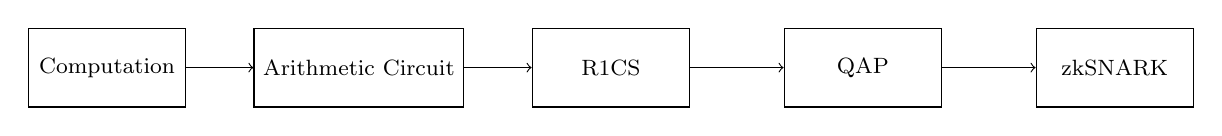
\begin{tikzpicture}[
    flow/.style={rectangle, minimum width=2cm, minimum height=1cm, text centered, draw=black,font=\footnotesize},
    scale=0.8
  ]
    \node[flow] (comp) at (0, 0) {Computation};
    \node[flow] (alg) at (4, 0) {Arithmetic Circuit};
    \node[flow] (r1cs) at (8, 0) {R1CS};
    \node[flow] (qap) at (12, 0) {QAP};
    \node[flow] (zk) at (16, 0) {zkSNARK};

    \draw[->] (comp) -- (alg);
    \draw[->] (alg) -- (r1cs);
    \draw[->] (r1cs) -- (qap);
    \draw[->] (qap) -- (zk);


  \end{tikzpicture}
  \caption{Steps of zk-SNARK}
  \label{fig:zkp:zksnark_flow}
\end{figure}

\subsubsection{Arithmetic circuits}
\label{zkp:snarks:circuits}

An arithmetic circuit $C$ over a finite field $\F_p$ is a circuit that contains
only addition and multiplication gates. It takes as inputs elements in $\F_p$ and its gates output elements in $\F_p$~\cite{184425, zcash}. The outputs are determined by the inputs which pass through the gates where their values are changed accordingly. Any program  can be reduced to  an arithmetic circuit~\cite{pankova_succinct_2013, 10.1007/978-3-642-40084-1_6} and normally the circuit is associated to the function it computes; the outsource function the prover works upon.

A legal or a valid assignment for an arithmetic circuit $C$ is a tuple $(c_1, c_2, \dots, c_n) \in \F_p$ such that $C(c_1, c_2, \dots, c_k) = (c_{k+1}, c_2, \dots, c_n)$ where $k$ is the number of all input and $n - k$ the number of all outputs of the circuit. Given a circuit evaluation, the task of the prover is to convince the verifier that there exist evaluations of intermediate gates such that the circuit indeed produces such an output with such an input~\cite{pankova_succinct_2013}. For example, if Alice wants to prove to Bob that she knows $c_1, c_2, c_3 \in \F_p$, such as $(c_{1}c_{2})(c_1 + c_3) = 7$, first she has to encode the computation to an arithmetic circuit $C$ (the presentation of $C$ is shown in Figure~\ref{fig:zkp:circuit}). Then she wants to prove that she knows a valid assignment $(c_1, c_2, c_3, c_4, c_5)$, where $c_4 = c_{1}c_{2}$ and $c_5 = c_{4}(c_1 + c_3)$, such that $c_5 = 7$.

\begin{figure}[ht!]
  \center
  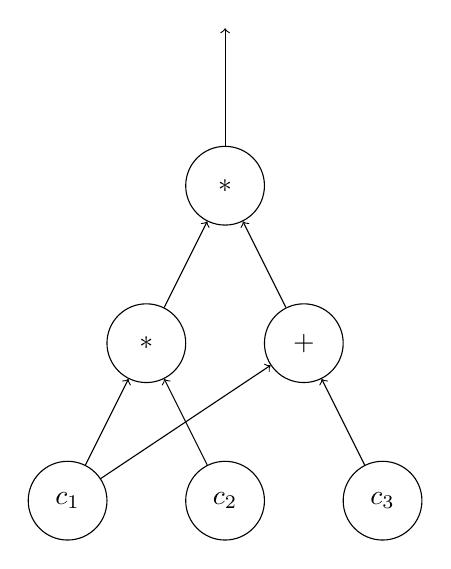
\begin{tikzpicture}[
        gate/.style={
        circle,
        minimum size=1cm,
        draw
      },
      node distance=2cm
    ]

    \node[gate] (c1) at (0, 0) {$c_1$};
    \node[gate] (c2) at (2, 0) {$c_2$};
    \node[gate] (c_3) at (4, 0) {$c_3$};

    \node[gate] (g1) at (1, 2) {$*$};
    \node[gate] (_g) at (3, 2) {$+$};

    \node[gate] (g2) at (2, 4) {$*$};

    \draw[->] (c1) -- (g1);
    \draw[->] (c1) -- (_g);
    \draw[->] (c2) -- (g1);

    \draw[->] (c_3) -- (_g);

    \draw[->] (g1) -- (g2);
    \draw[->] (_g) -- (g2);

    \draw[->] (g2) -- ++(0, 2);

  \end{tikzpicture}
  \caption{A simple arithmetic circuit}
  \label{fig:zkp:circuit}
\end{figure}

\subsubsection[Quadratic Arithmetic Program (QAP)]{Quadratic Arithmetic Program (QAP)~\cite{zksnark_basics, zcash_snarks}}
\label{zkp:snarks:qap}

Geranno et. al~\cite{ggpr} showed how to encode efficiently computation as quadratic programs called Quadratic Arithmetic Programs (QAP) to obtain zk-SNARKs. QAPs play an important role as they enable the prover to construct the proof $\pi$ claiming that she knows a valid assignment of a circuit $C$.

A  QAP $Q(C) = (L, R, O, T)$ for a given circuit $C$ is a set of three polynomials

\begin{align*}
  L = \sum_{i=1}^{m}c_{i}L_{i} && R = \sum_{i=1}^{m}c_{i}R_{i} && O = \sum_{i=1}^{m}c_{i}O_{i} && (m \geq n)
\end{align*}

and a target polynomial $T$ such that $T$ divides the polynomial:

\begin{equation*}
  P = LR - O
\end{equation*}

if and only if $(c_1, c_2, \dots, c_n)$ is a valid assignment for $C$. The prover constructs the polynomial for its proof $\pi$ and the verifier check the divisibility of $P$ by $T$. Equivalent, $P = TH$ for some polynomial $H$.

To translate the $C$ into a QAP the wires and gates must be labeled in a specific way:

\begin{itemize}
  \item Each multiplication gate has exactly two input wires: left and right wire
  \item Each multiplication gate has a unique label
  \item Addition gates are not labeled
  \item Outgoing wires to more than one gate are labeled as one wire
  \item Outgoing wires from an addition gate to a multiplication gate are not labeled; the inputs of an addition gate go directly to the multiplication gate
\end{itemize}

A label assignment of circuit of Figure~\ref{fig:zkp:circuit} is shown in Figure~\ref{fig:zkp:circuit_label}.

\begin{figure}[ht!]
  \center
  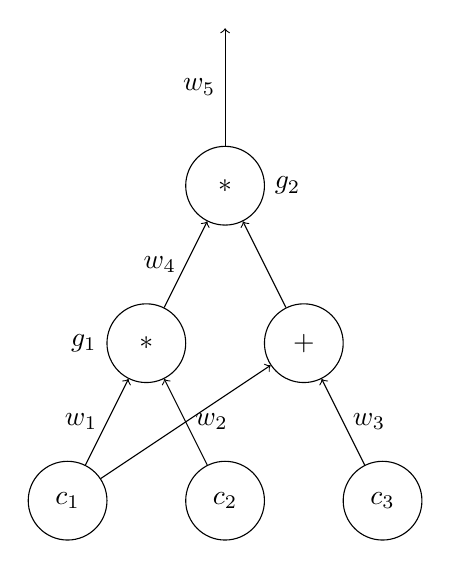
\begin{tikzpicture}[
        gate/.style={
        circle,
        minimum size=1cm,
        draw
      },
      node distance=2cm
    ]

    \node[gate] (c1) at (0, 0) {$c_1$};
    \node[gate] (c2) at (2, 0) {$c_2$};
    \node[gate] (c_3) at (4, 0) {$c_3$};

    \node[gate, label={left:$g_1$}] (g1) at (1, 2) {$*$};
    \node[gate] (_g) at (3, 2) {$+$};

    \node[gate, label={right:$g_2$}] (g2) at (2, 4) {$*$};

    \draw[->] (c1) -- (g1) node[midway,left] {$w_1$};
    \draw[->] (c1) -- (_g);
    \draw[->] (c2) -- (g1) node[midway,right] {$w_2$};

    \draw[->] (c_3) -- (_g) node[midway,right] {$w_3$};

    \draw[->] (g1) -- (g2) node[midway,left] {$w_4$};
    \draw[->] (_g) -- (g2);

    \draw[->] (g2) -- ++(0, 2) node[midway,left] {$w_5$};

  \end{tikzpicture}
  \caption{Circuit label assignment}
  \label{fig:zkp:circuit_label}
\end{figure}

The circuit is ready to be transformed to a QAP. Let $M$ is the set of the index of the multiplication gates and $W$ the set of input and output wires. The points in $M$ are called target points. For each gate $g \in M$ we construct a set of left, right, and output polynomials as follows: for each wire a polynomial is constructed in such way that it evaluates at zero on all target point expect the ones that correspond to the multiplication gate.

\textbf{QAP construction of circuit of Figure~\ref{fig:zkp:circuit_label}}: Gate $g_1$, with target point $1$, has $w_1$ as left wire, $w_2$ as right wire and $w_4$ as output label. Thus, we construct $L_1 = R_2 = O_4 = 2 - x$ as the polynomial on point $1$ corresponding to $g_1$ is one and zero on point $2$ corresponding to $g_2$. Similar, for gate $g_2$ $L_4 = R_1 = R_3 = O_5 = x - 1$. Note that the wires $w_2$ and $w_3$ are both right inputs of $g_2$.

The wire polynomials:

\begin{align*}
  L_1 = (2 - x) && L_2 = 0 && L_3 = 0 && L_4 = (x - 1) && L_5 = 0
\end{align*}
\begin{align*}
  R_1 = (x - 1) && R_2 = (2 - x) && R_3 = (x - 1) && R_4 = 0 && R_5 = 0
\end{align*}
\begin{align*}
  O_1 = 0 && O_2 = 0 && O_3 = 0 && O_4 = (2 - x) && O_5 = (x - 1)
\end{align*}

The total left, right and output polynomials:

\begin{align*}
  L &= \sum_{i=1}^{5}c_{i}L_{i} & R &= \sum_{i=1}^{5}c_{i}R_{i} & O &= \sum_{i=1}^{5}c_{i}O_{i} \\
    &= c_1L_1 + c_4L_4 & &= c_1R_1 + c_2R_2 + c_3R_3 & &= c_4O_4 + c_5O_5 \\
    &= c_1(2 - x) + c_4(x - 1) & &= c_1(x - 1) + c_2(2 - x) + c_3(x - 1) & &= c_4(2 - x) + c_5(x - 1)
\end{align*}

If we evaluate these polynomials at target points $1$ and $2$ we get:

\begin{align*}
  P(1) &= L(1)R(1) - O(1) & P(2) &= L(2)R(2) - O(2) \\
       &= c_1c_2 - c_4 & &=c_4(c_1 + c_3) - c_5
\end{align*}

Hence, $T(x) = (x - 1)(x - 2)$ divides $P(x)$ if and only $1, 2$ are roots of $P(x)$; $(c_1, c_2, \dots, c_5)$ is a valid assignment for $C$.
